\chapter{Testing}
\label{apendix_testing}
\settocdepth{chapter}


\section{Test Cases}
\label{test_cases}


\begin{longtable}{@{\extracolsep{\fill}}
                |L{0.30\linewidth}
                |L{0.65\linewidth}|@{}}
\hline
\rowcolor{Gray}
\textbf{ID} & TC1 - all\\
\hline
\textbf{Name} & Log in \\
\hline
\textbf{Requirement to be tested} & US.03\\
\hline
\textbf{Preconditions} & Have a Facebook user, or need to register a user \\
\hline
\textbf{Description} & Try to log in with Facebook if you own this, or create a user and log in \\
\hline
\textbf{Acceptance criteria} & A user must be able to log in, get feedback after log in, stay logged in after refreshing page and be able to log out
 \\
\hline
\textbf{Test status} & \cellcolor[HTML]{b6d7a8}Passed \\
\hline
\caption{Test Case 1}
\label{TC1}
\end{longtable}


\begin{longtable}{@{\extracolsep{\fill}}
                |L{0.30\linewidth}
                |L{0.65\linewidth}|@{}}
\hline
\rowcolor{Gray}
\textbf{ID} & TC2 - all \\
\hline
\textbf{Name} & Add new roles to profile \\
\hline
\textbf{Requirement to be tested} & US.03 \\
\hline
\textbf{Preconditions} & Be logged in \\
\hline
\textbf{Description} & Log inn and go to my page to add new members to your profile\\
\hline
\textbf{Acceptance criteria} &  Members are successfully created and appears on the profile  \\
\hline
\textbf{Test status} & \cellcolor[HTML]{b6d7a8}Passed\\
\hline
\caption{Test Case 2}
\label{TC2}
\end{longtable}

\begin{longtable}{@{\extracolsep{\fill}}
                |L{0.30\linewidth}
                |L{0.65\linewidth}|@{}}
\hline
\rowcolor{Gray}
\textbf{ID} & TC3 - all \\
\hline
\textbf{Name} & Change between roles \\
\hline
\textbf{Requirement to be tested} & US.03\\
\hline
\textbf{Preconditions} & Be logged in and have multiple roles connected to profile\\
\hline
\textbf{Description} & Change user with the menu in the navbar\\
\hline
\textbf{Acceptance criteria} &  The new active user is shown on the profile page \\
\hline
\textbf{Test status} & \cellcolor[HTML]{b6d7a8}Passed \\
\hline
\caption{Test Case 3}
\label{TC3}
\end{longtable}


\begin{longtable}{@{\extracolsep{\fill}}
                |L{0.30\linewidth}
                |L{0.65\linewidth}|@{}}
\hline
\rowcolor{Gray}
\textbf{ID} & TC4 - provider\\
\hline
\textbf{Name} & Connect profile to provider \\
\hline
\textbf{Requirement to be tested} & US.03\\
\hline
\textbf{Preconditions} & Have a registered profile and be logged in \\
\hline
\textbf{Description} & Go to my page and click the button "Administrer arrangører" to add new provider \\
\hline
\textbf{Acceptance criteria} &  The provider selected is shown on my page \\
\hline
\textbf{Test status} & \cellcolor[HTML]{b6d7a8}Passed  \\
\hline
\caption{Test Case 4}
\label{TC4}
\end{longtable}


\begin{longtable}{@{\extracolsep{\fill}}
                |L{0.30\linewidth}
                |L{0.65\linewidth}|@{}}
\hline
\rowcolor{Gray}
\textbf{ID} & TC5 - parent and provider \\
\hline
\textbf{Name} & Create activity \\
\hline
\textbf{Requirement to be tested} & PA.02, PR.00, PR.02, PR.03\\
\hline
\textbf{Preconditions} & Have an profile account and be logged in \\
\hline
\textbf{Description} & Click "Opprett aktivitet" in navbar and add all information needed in the form, save the form \\
\hline
\textbf{Acceptance criteria} &  The activity created is shown on the "Aktiviteter" page \\
\hline
\textbf{Test status} & \cellcolor[HTML]{b6d7a8}Passed  \\
\hline
\caption{Test Case 5}
\label{TC5}
\end{longtable}



\begin{longtable}{@{\extracolsep{\fill}}
                |L{0.30\linewidth}
                |L{0.65\linewidth}|@{}}
\hline
\rowcolor{Gray}
\textbf{ID} & TC6 - parent and provider \\
\hline
\textbf{Name} & Create activity based on Facebook \\
\hline
\textbf{Requirement to be tested} & PA.02, PR.00, PR.02, PR.03, SM.03 \\
\hline
\textbf{Preconditions} & Have an user account and be logged in \\
\hline
\textbf{Description} &  Click "Opprett aktivitet" in navbar and add an arragement you are attending or hosting from Facebook, save the form \\
\hline
\textbf{Acceptance critera} &  Check that the activity is shown on the "Aktiviteter" page and that the Facebook information is shown together with the Facebook logo. \\
\hline
\textbf{Test status} & \cellcolor[HTML]{b6d7a8}Passed  \\
\hline
\caption{Test Case 6}
\label{TC6}
\end{longtable}

\begin{longtable}{@{\extracolsep{\fill}}
                |L{0.30\linewidth}
                |L{0.65\linewidth}|@{}}
\hline
\rowcolor{Gray}
\textbf{ID} & TC7 - parent and provider \\
\hline
\textbf{Name} & Create activity with Instagram picture \\
\hline
\textbf{Requirement to be tested} & PA.02, PR.00, PR.02, PR.03\\
\hline
\textbf{Preconditions} & Have an profile account and be logged in \\
\hline
\textbf{Description} & Click "Opprett aktivitet" in navbar and add all information needed in the form, make sure to add a image from Instagram, save the form \\
\hline
\textbf{Acceptance criteria} &  The activity created is shown on the "Aktiviteter" page, check if the Instagram image is visible \\
\hline
\textbf{Test status} &  \cellcolor[HTML]{b6d7a8}Passed \\
\hline
\caption{Test Case 7}
\label{TC7}
\end{longtable}

\begin{longtable}{@{\extracolsep{\fill}}
                |L{0.30\linewidth}
                |L{0.65\linewidth}|@{}}
\hline
\rowcolor{Gray}
\textbf{ID} & TC8 - parent and provider \\
\hline
\textbf{Name} & See activities I have created \\
\hline
\textbf{Requirement to be tested} & \\
\hline
\textbf{Preconditions} & Have an profile account and be logged in, have created some activities \\
\hline
\textbf{Description} & Go to my page and see if any of the activities created in TC5 (\ref{TC5}), TC6 (\ref{TC6}) and TC7 (\ref{TC7}) is available\\
\hline
\textbf{Acceptance criteria} &  The activities is shown on my page \\
\hline
\textbf{Test status} & \cellcolor[HTML]{b6d7a8}Passed  \\
\hline
\caption{Test Case 8}
\label{TC8}
\end{longtable}


\begin{longtable}{@{\extracolsep{\fill}}
                |L{0.30\linewidth}
                |L{0.65\linewidth}|@{}}
\hline
\rowcolor{Gray}
\textbf{ID} & TC9 - all \\
\hline
\textbf{Name} & Find activities \\
\hline
\textbf{Requirement to be tested} & US.00, US.01, US.06, US.07, CH.00, CH.03, PA.00, PA.01 \\
\hline
\textbf{Preconditions} &  None \\
\hline
\textbf{Description} & Go to all activities page and try to search and use filter to find activities that fits you  \\
\hline
\textbf{Acceptance criteria} & The user should be able to view all activities, and only the activities matching the filters appears  \\
\hline
\textbf{Test status} &  \cellcolor[HTML]{b6d7a8}Passed \\
\hline
\caption{Test Case 9}
\label{TC9}
\end{longtable}


\begin{longtable}{@{\extracolsep{\fill}}
                |L{0.30\linewidth}
                |L{0.65\linewidth}|@{}}
\hline
\rowcolor{Gray}
\textbf{ID} & TC10 - all \\
\hline
\textbf{Name} & One activity \\
\hline
\textbf{Requirement to be tested} & US.01, PA.04, PR.01 \\
\hline
\textbf{Preconditions} & None \\
\hline
\textbf{Description} &  Find and click one activity and check if the information is easily accessible and explanatory\\
\hline
\textbf{Acceptance criteria} &  The modal opens and the information is presented \\
\hline
\textbf{Test status} &  \cellcolor[HTML]{b6d7a8}Passed \\
\hline
\caption{Test Case 10}
\label{TC10}
\end{longtable}


\begin{longtable}{@{\extracolsep{\fill}}
                |L{0.30\linewidth}
                |L{0.65\linewidth}|@{}}
\hline
\rowcolor{Gray}
\textbf{ID} & TC11 - all \\
\hline
\textbf{Name} &  Attend an activity \\
\hline
\textbf{Requirement to be tested} & US.04, CH.01\\
\hline
\textbf{Preconditions} & Have an user account and be logged in  \\
\hline
\textbf{Description} &  Find and open an activity and press the attend button\\
\hline
\textbf{Acceptance criteria} &  The modal opens, the button changes from "Meld på" to "Meld av" \\
\hline
\textbf{Test status} &  \cellcolor[HTML]{b6d7a8}Passed \\
\hline
\caption{Test Case 11}
\label{TC11}
\end{longtable}

\begin{longtable}{@{\extracolsep{\fill}}
                |L{0.30\linewidth}
                |L{0.65\linewidth}|@{}}
\hline
\rowcolor{Gray}
\textbf{ID} & TC12 - all \\
\hline
\textbf{Name} & See activities I am attending \\
\hline
\textbf{Requirement to be tested} & US.04, CH.01\\
\hline
\textbf{Preconditions} & Have an profile account and be logged in, are attending some activities \\
\hline
\textbf{Description} & Go to my page and see if any if the activity attending in TC11 (\ref{TC11}) is shown\\
\hline
\textbf{Acceptance criteria} &  The activity attending is shown on my page \\
\hline
\textbf{Test status} & \cellcolor[HTML]{b6d7a8}Passed  \\
\hline
\caption{Test Case 12}
\label{TC12}
\end{longtable}


\begin{longtable}{@{\extracolsep{\fill}}
                |L{0.30\linewidth}
                |L{0.65\linewidth}|@{}}
\hline
\rowcolor{Gray}
\textbf{ID} & TC13 - all \\
\hline
\textbf{Name} & Find providers \\
\hline
\textbf{Requirement to be tested} &  \\
\hline
\textbf{Preconditions} &  None \\
\hline
\textbf{Description} & Go to all provider page and try to search and use filter to find provider that fits you  \\
\hline
\textbf{Acceptance criteria} & The user should be able to view all providers, and only the providers matching the filters appears  \\
\hline
\textbf{Test status} & \cellcolor[HTML]{b6d7a8}Passed  \\
\hline
\caption{Test Case 13}
\label{TC13}
\end{longtable}


\begin{longtable}{@{\extracolsep{\fill}}
                |L{0.30\linewidth}
                |L{0.65\linewidth}|@{}}
\hline
\rowcolor{Gray}
\textbf{ID} & TC14 - all \\
\hline
\textbf{Name} & Follow providers \\
\hline
\textbf{Requirement to be tested} &  \\
\hline
\textbf{Preconditions} &  Have an profile account and be logged in \\
\hline
\textbf{Description} & Go to all provider page and click follow provider button \\
\hline
\textbf{Acceptance criteria} & The button changes to unfollow provider  \\
\hline
\textbf{Test status} &  \cellcolor[HTML]{b6d7a8}Passed \\
\hline
\caption{Test Case 14}
\label{TC14}
\end{longtable}

\begin{longtable}{@{\extracolsep{\fill}}
                |L{0.30\linewidth}
                |L{0.65\linewidth}|@{}}
\hline
\rowcolor{Gray}
\textbf{ID} & TC15 - all \\
\hline
\textbf{Name} & See providers I am attending \\
\hline
\textbf{Requirement to be tested} & \\
\hline
\textbf{Preconditions} & Have an profile account and be logged in, are following some providers \\
\hline
\textbf{Description} & Go to my page and see if any if the providers you are following in TC14 (\ref{TC14}) is shown\\
\hline
\textbf{Acceptance criteria} &  The provider you are following is shown on my page \\
\hline
\textbf{Test status} & \cellcolor[HTML]{b6d7a8}Passed  \\
\hline
\caption{Test Case 15}
\label{TC15}
\end{longtable}

\section{Errors Detected During Pre-Focus Group Families}
\label{errors_detected_during_pre-focus_group_families}

\subsubsection{Front page}
\begin{longtable}{@{\extracolsep{\fill}}
                |L{0.40\linewidth}
                |L{0.10\linewidth}
                |L{0.10\linewidth}
                |L{0.15\linewidth}
                |L{0.15\linewidth}|@{}}
                
\hline
\rowcolor{Gray}
\textbf{Description} & \textbf{Likelihood {\footnotesize (1-9)}} & \textbf{Impact {\footnotesize (1-9)}} & \textbf{Importance and Risk{\footnotesize (Likelihood * Impact)}} & \textbf{Correction Status} \\
\hline
Unnecessary console log on front page & 1 & 1 & \cellcolor[HTML]{b6d7a8}1 & Fixed \\
\hline
Sort activities on front page based on date & 5 & 6 & \cellcolor[HTML]{FFD966}30 & Fixed \\
\hline
Activities that has been should not be visible & 6 & 6 & \cellcolor[HTML]{FFD966}36 & Fixed \\
\hline
\caption{Software Inspection Errors - Front Page}
\label{Errors_Software_Inspection_4}
\end{longtable}


\subsubsection{Activities}
\begin{longtable}{@{\extracolsep{\fill}}
                |L{0.40\linewidth}
                |L{0.10\linewidth}
                |L{0.10\linewidth}
                |L{0.15\linewidth}
                |L{0.15\linewidth}|@{}}
                
\hline
\rowcolor{Gray}
\textbf{Description} & \textbf{Likelihood {\footnotesize (1-9)}} & \textbf{Impact {\footnotesize (1-9)}} & \textbf{Importance and Risk {\footnotesize (Likelihood * Impact)}} & \textbf{Correction Status} \\
\hline
Unnecessary console log on front page & 1 & 1 & \cellcolor[HTML]{b6d7a8}1 & Fixed \\
\hline
Should have margin between last activity card and footer & 2 & 2 & \cellcolor[HTML]{b6d7a8}4 & Fixed \\
\hline
Change input fields to be same on all pages & 1 & 3 & \cellcolor[HTML]{b6d7a8}3 & Fixed \\
\hline
Calendar should be in Norwegian & 1 & 1 & \cellcolor[HTML]{b6d7a8}1 & Fixed \\
\hline
\caption{Software Inspection Errors - Activities}
\label{Errors_Software_Inspection_5}
\end{longtable}


\subsubsection{Activity Modal}
\begin{longtable}{@{\extracolsep{\fill}}
                |L{0.40\linewidth}
                |L{0.10\linewidth}
                |L{0.10\linewidth}
                |L{0.15\linewidth}
                |L{0.15\linewidth}|@{}}
                
\hline
\rowcolor{Gray}
\textbf{Description} & \textbf{Likelihood {\footnotesize (1-9)}} & \textbf{Impact {\footnotesize (1-9)}} & \textbf{Importance and Risk {\footnotesize (Likelihood * Impact)}} & \textbf{Correction Status} \\
\hline
Year should be displayed below date & 1 & 2 & \cellcolor[HTML]{b6d7a8}2 & Fixed \\
\hline
Comment does not show immediately & 7 & 7 & \cellcolor[HTML]{FFD966}49 & Fixed \\
\hline
The modal becomes large if information text is long, should have a show more button  & 5 & 3 & \cellcolor[HTML]{b6d7a8}15 & Fixed \\
\hline
Remove ";" which stands after the star on rate an activity  & 1 & 1 & \cellcolor[HTML]{b6d7a8}1 & Fixed \\
\hline
\caption{Software Inspection Errors - Activity Modal}
\label{Errors_Software_Inspection_6}
\end{longtable}


\subsubsection{Create Activity}
\begin{longtable}{@{\extracolsep{\fill}}
                |L{0.40\linewidth}
                |L{0.10\linewidth}
                |L{0.10\linewidth}
                |L{0.15\linewidth}
                |L{0.15\linewidth}|@{}}
                
\hline
\rowcolor{Gray}
\textbf{Description} & \textbf{Likelihood {\footnotesize (1-9)}} & \textbf{Impact {\footnotesize (1-9)}} & \textbf{Importance and Risk {\footnotesize (Likelihood * Impact)}} & \textbf{Correction Status} \\
\hline
The import from Facebook box does not always show & 3 & 9 & \cellcolor[HTML]{FFD966}27 & Not fixed, can not reproduce \\
\hline
Instagram does not work & 7 & 9 & \cellcolor[HTML]{e06666}63 & Fixed \\
\hline
Images from Facebook does not appear the first time, appears when activity is edited & 5 & 7 & \cellcolor[HTML]{FFD966}35 & Fixed \\
\hline
Title has wrong font & 1 & 2 & \cellcolor[HTML]{b6d7a8}2 & Fixed \\
\hline
Activity type should be required when creating & 3 & 7 & \cellcolor[HTML]{FFD966}21 & Not fixed, argument is proof of concept. \\
\hline
\caption{Software Inspection Errors - Create Activity}
\label{Errors_Software_Inspection_7}
\end{longtable}


\subsubsection{Provider}
\begin{longtable}{@{\extracolsep{\fill}}
                |L{0.40\linewidth}
                |L{0.10\linewidth}
                |L{0.10\linewidth}
                |L{0.15\linewidth}
                |L{0.15\linewidth}|@{}}
                
\hline
\rowcolor{Gray}
\textbf{Description} & \textbf{Likelihood {\footnotesize (1-9)}} & \textbf{Impact {\footnotesize (1-9)}} & \textbf{Importance and Risk {\footnotesize (Likelihood * Impact)}} & \textbf{Correction Status} \\
\hline
Alginment between filter, providers and load more button is not correct & 1 & 2 & \cellcolor[HTML]{b6d7a8}2 & Fixed \\
\hline
Follow provider button should have margin around & 1 & 2 & \cellcolor[HTML]{b6d7a8}2 & Fixed \\
\hline
Fix styling for one provider & 2 & 2 & \cellcolor[HTML]{b6d7a8}4 & Fixed \\
\hline
Change input fields to be same on all pages & 1 & 3 & \cellcolor[HTML]{b6d7a8}3 & Fixed \\
\hline
\caption{Software Inspection Errors - Provider}
\label{Errors_Software_Inspection_8}
\end{longtable}



\subsubsection{Administer Provider}
\begin{longtable}{@{\extracolsep{\fill}}
                |L{0.40\linewidth}
                |L{0.10\linewidth}
                |L{0.10\linewidth}
                |L{0.15\linewidth}
                |L{0.15\linewidth}|@{}}
                
\hline
\rowcolor{Gray}
\textbf{Description} & \textbf{Likelihood {\footnotesize (1-9)}} & \textbf{Impact {\footnotesize (1-9)}} & \textbf{Importance and Risk {\footnotesize (Likelihood * Impact)}} & \textbf{Correction Status} \\
\hline
Navbar does not show that the user is logged in on this page & 8 & 9 & \cellcolor[HTML]{e06666}72 & Fixed \\
\hline
Buttons does not have right styling & 3 & 5 & \cellcolor[HTML]{b6d7a8}15 & Not fixed, due to time and proof of concept \\
\hline
\caption{Software Inspection Errors - Administer Provider}
\label{Errors_Software_Inspection_9}
\end{longtable}




\subsubsection{Register User}
\begin{longtable}{@{\extracolsep{\fill}}
                |L{0.40\linewidth}
                |L{0.10\linewidth}
                |L{0.10\linewidth}
                |L{0.15\linewidth}
                |L{0.15\linewidth}|@{}}
                
\hline
\rowcolor{Gray}
\textbf{Description} & \textbf{Likelihood {\footnotesize (1-9)}} & \textbf{Impact {\footnotesize (1-9)}} & \textbf{Importance and Risk {\footnotesize (Likelihood * Impact)}} & \textbf{Correction Status} \\
\hline
Two bottom checkboxes does not work, must click on text & 4 & 8 & \cellcolor[HTML]{FFD966}32 & Fixed \\
\hline
Should not have to create both user name and profile name & 2 & 7 & \cellcolor[HTML]{b6d7a8}14 & Fixed\\
\hline
\caption{Software Inspection Errors - Register User}
\label{Errors_Software_Inspection_10}
\end{longtable}


\subsubsection{My Page}
\begin{longtable}{@{\extracolsep{\fill}}
                |L{0.40\linewidth}
                |L{0.10\linewidth}
                |L{0.10\linewidth}
                |L{0.15\linewidth}
                |L{0.15\linewidth}|@{}}
                
\hline
\rowcolor{Gray}
\textbf{Description} & \textbf{Likelihood {\footnotesize (1-9)}} & \textbf{Impact {\footnotesize (1-9)}} & \textbf{Importance and Risk {\footnotesize (Likelihood * Impact)}} & \textbf{Correction Status} \\
\hline
E-mail and surname does not show when logged in with Facebook & 2 & 2 & \cellcolor[HTML]{b6d7a8}4 & Fixed \\
\hline
Phone number should not display none when not filled in & 3 & 4 & \cellcolor[HTML]{b6d7a8}12 & Fixed \\
\hline
Same picture on all profiles on one user & 4 & 4 & \cellcolor[HTML]{b6d7a8}16 & Fixed \\
\hline
Footer does not have margin when not attending any activity & 1 & 2 & \cellcolor[HTML]{b6d7a8}2 & Fixed \\
\hline
When user has only one profile the profile does not become active & 5 & 8 & \cellcolor[HTML]{FFD966}40 & Fixed\\
\hline
\caption{Software Inspection Errors - My Page}
\label{Errors_Software_Inspection_11}
\end{longtable}

\section{Focus Group With Providers and System Maintainers}
\label{workshop_with_providers_and_system_maintainers_appendix}
The workshop were held in Norwegian and therefore the notes are in Norwegian.

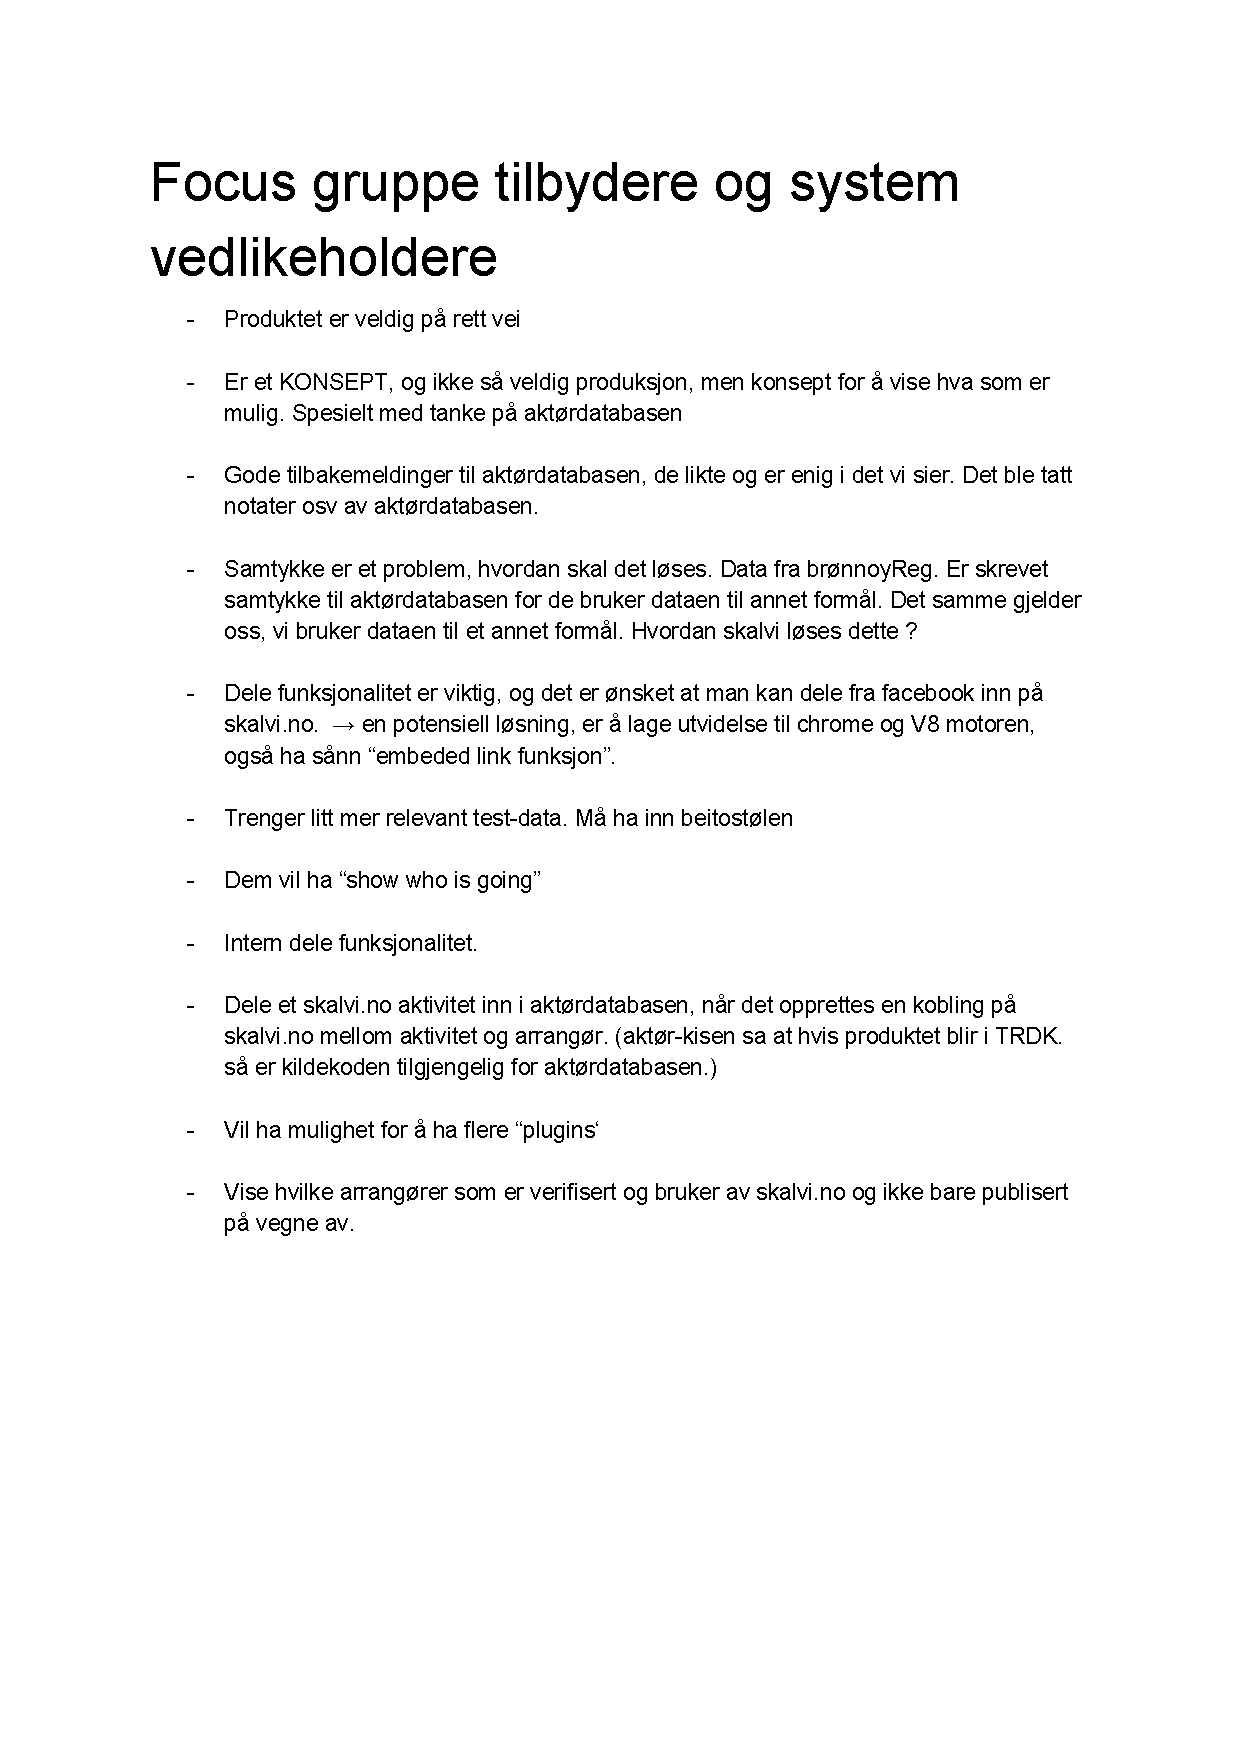
\includepdf[scale=0.9]{fig/focusgroup/FGProviders.pdf}



\section{Focus Group With Families}
\label{workshop_with_families_appendix}
The workshop were held in Norwegian and therefore the notes are in Norwegian.

%Children
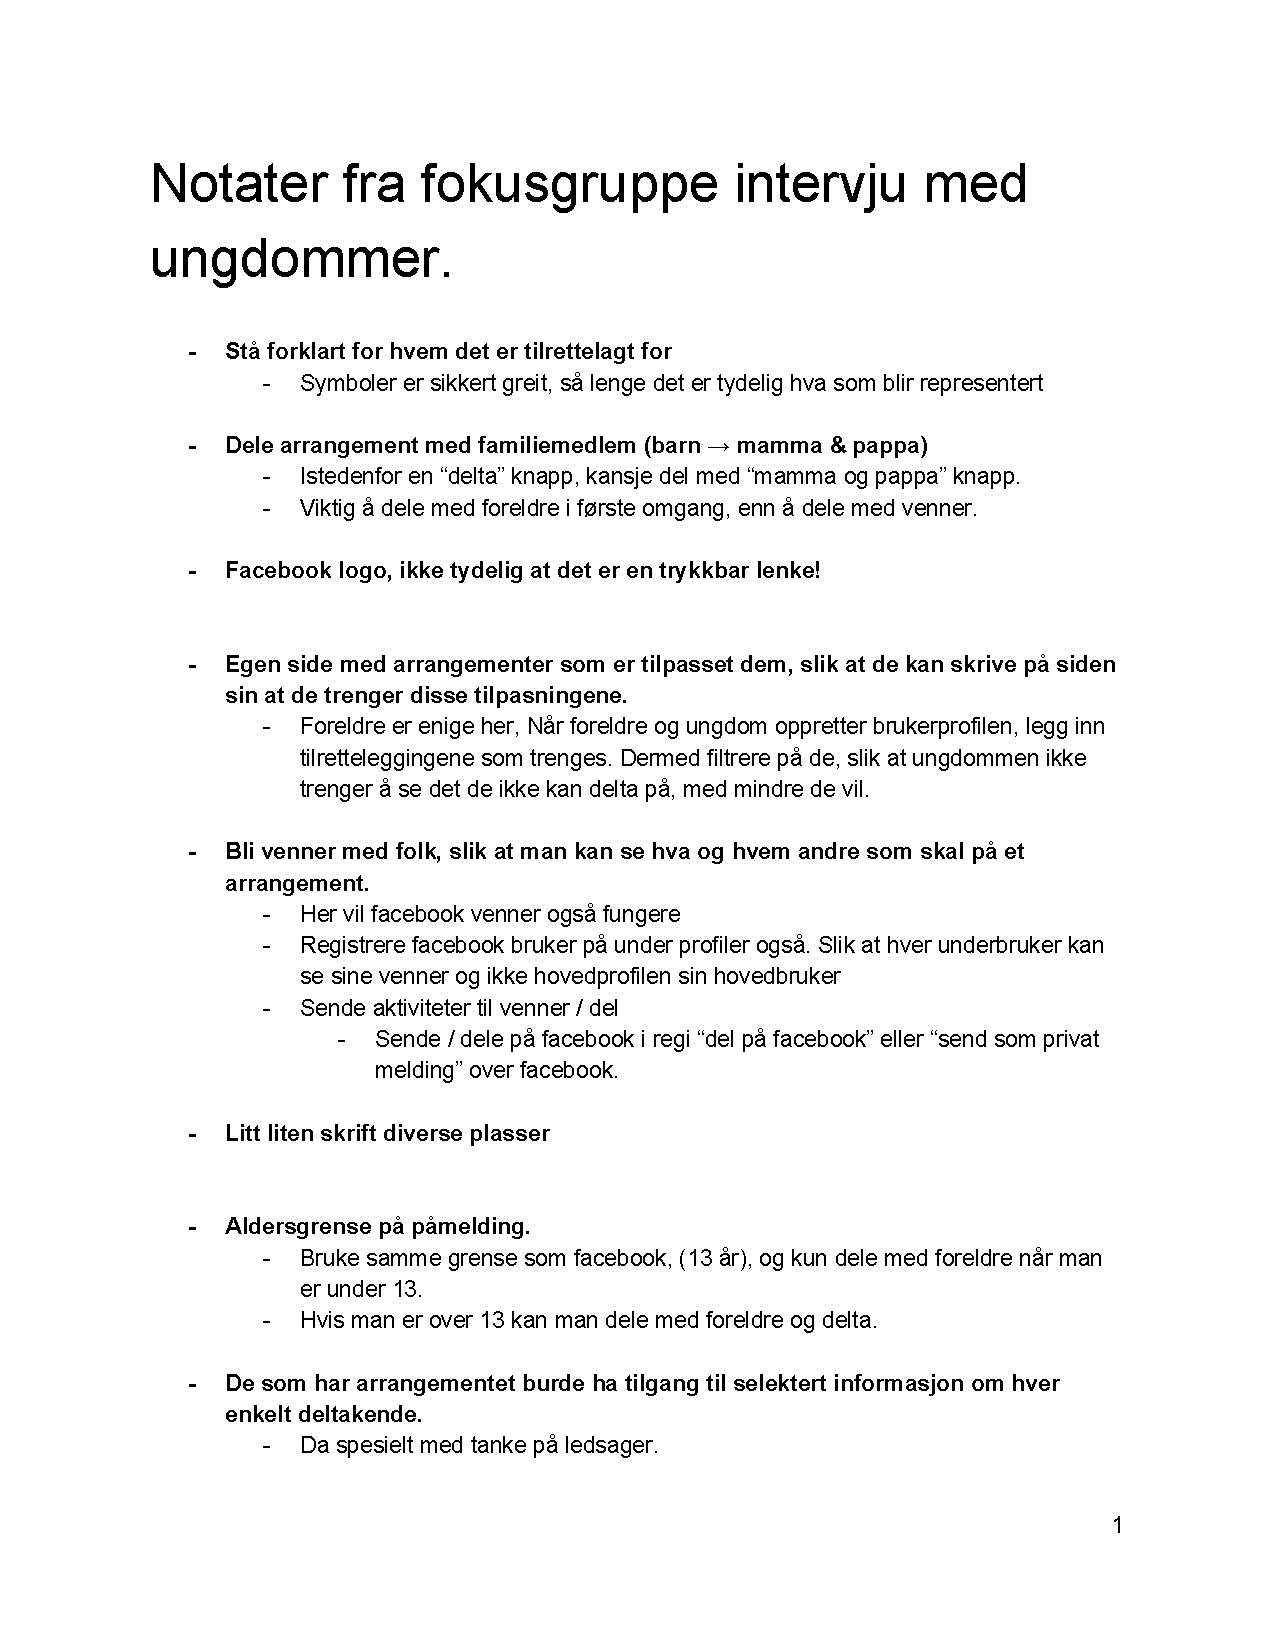
\includepdf[scale=0.9, pagecommand=\subsection{Children}]{fig/focusgroup/FGChildren_1.pdf}

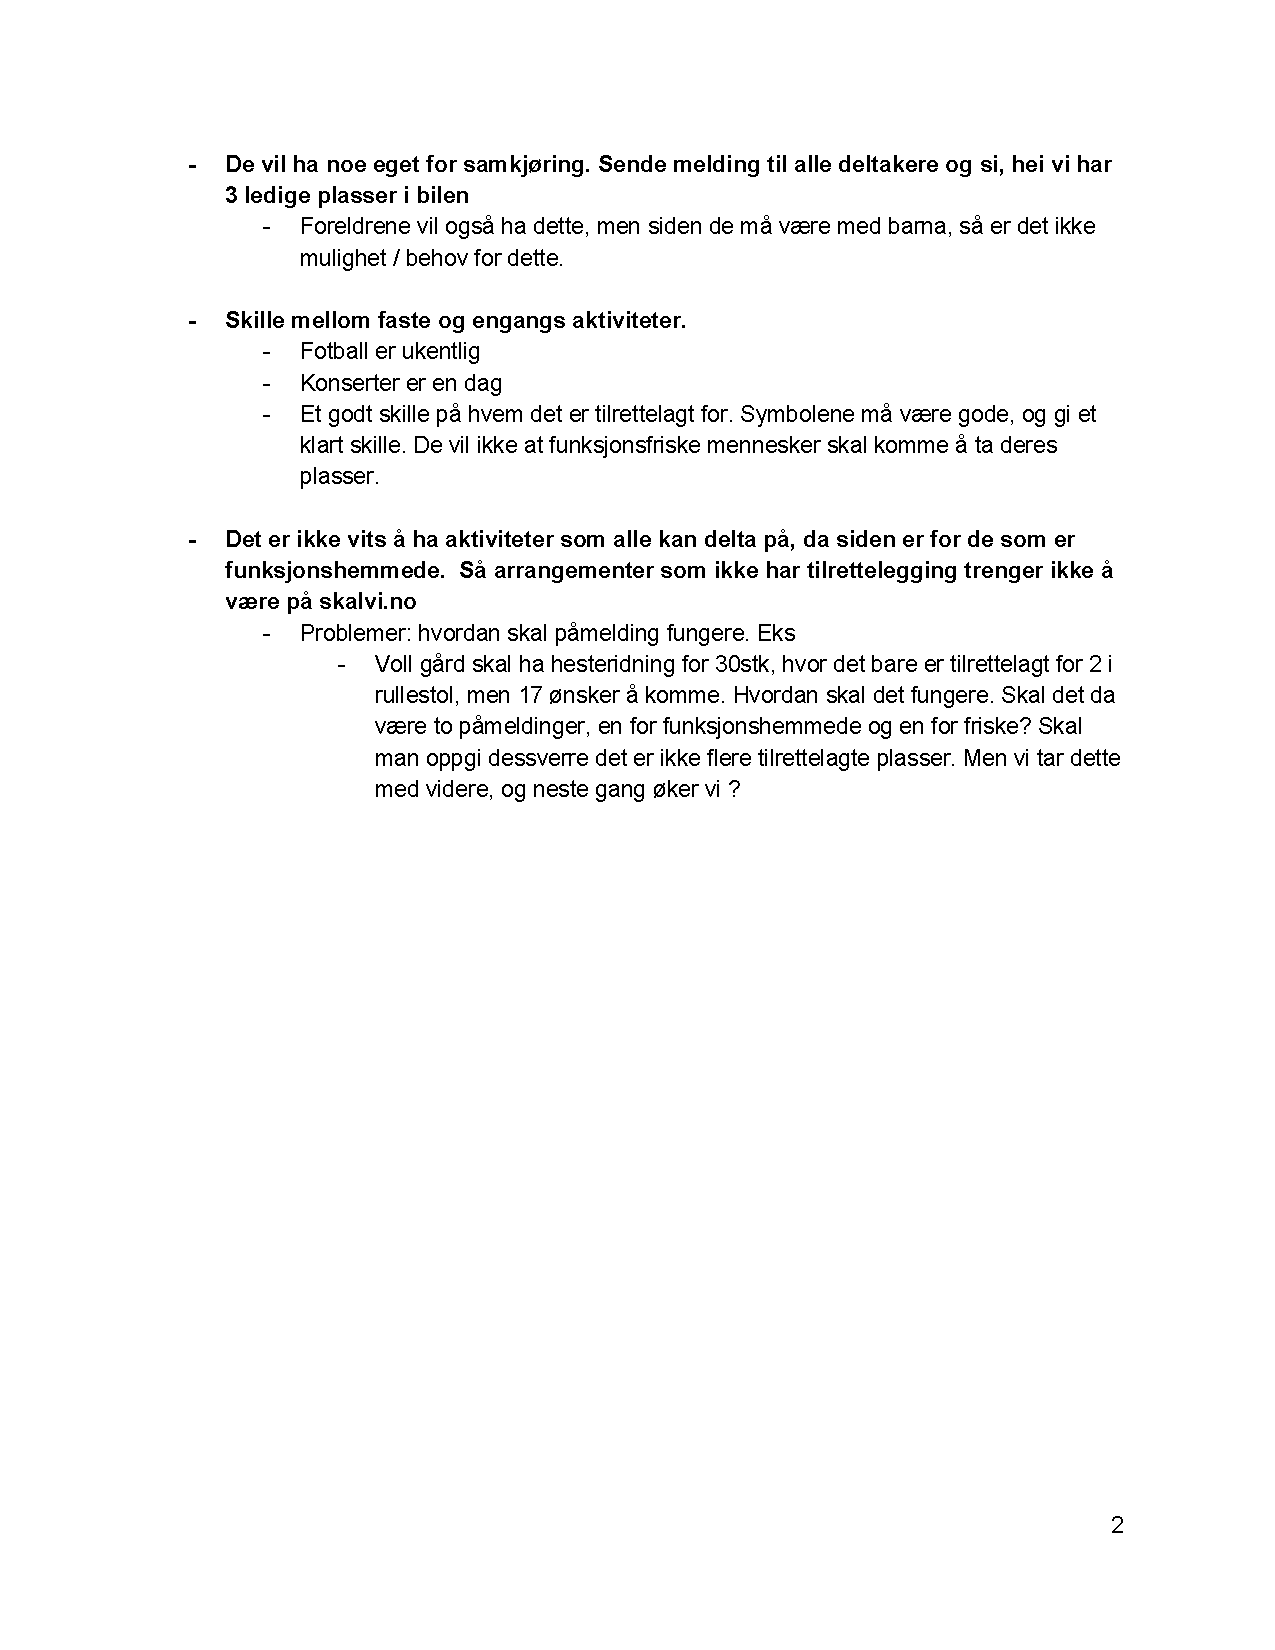
\includepdf[scale=0.9]{fig/focusgroup/FGChildren_2.pdf}

%Parents
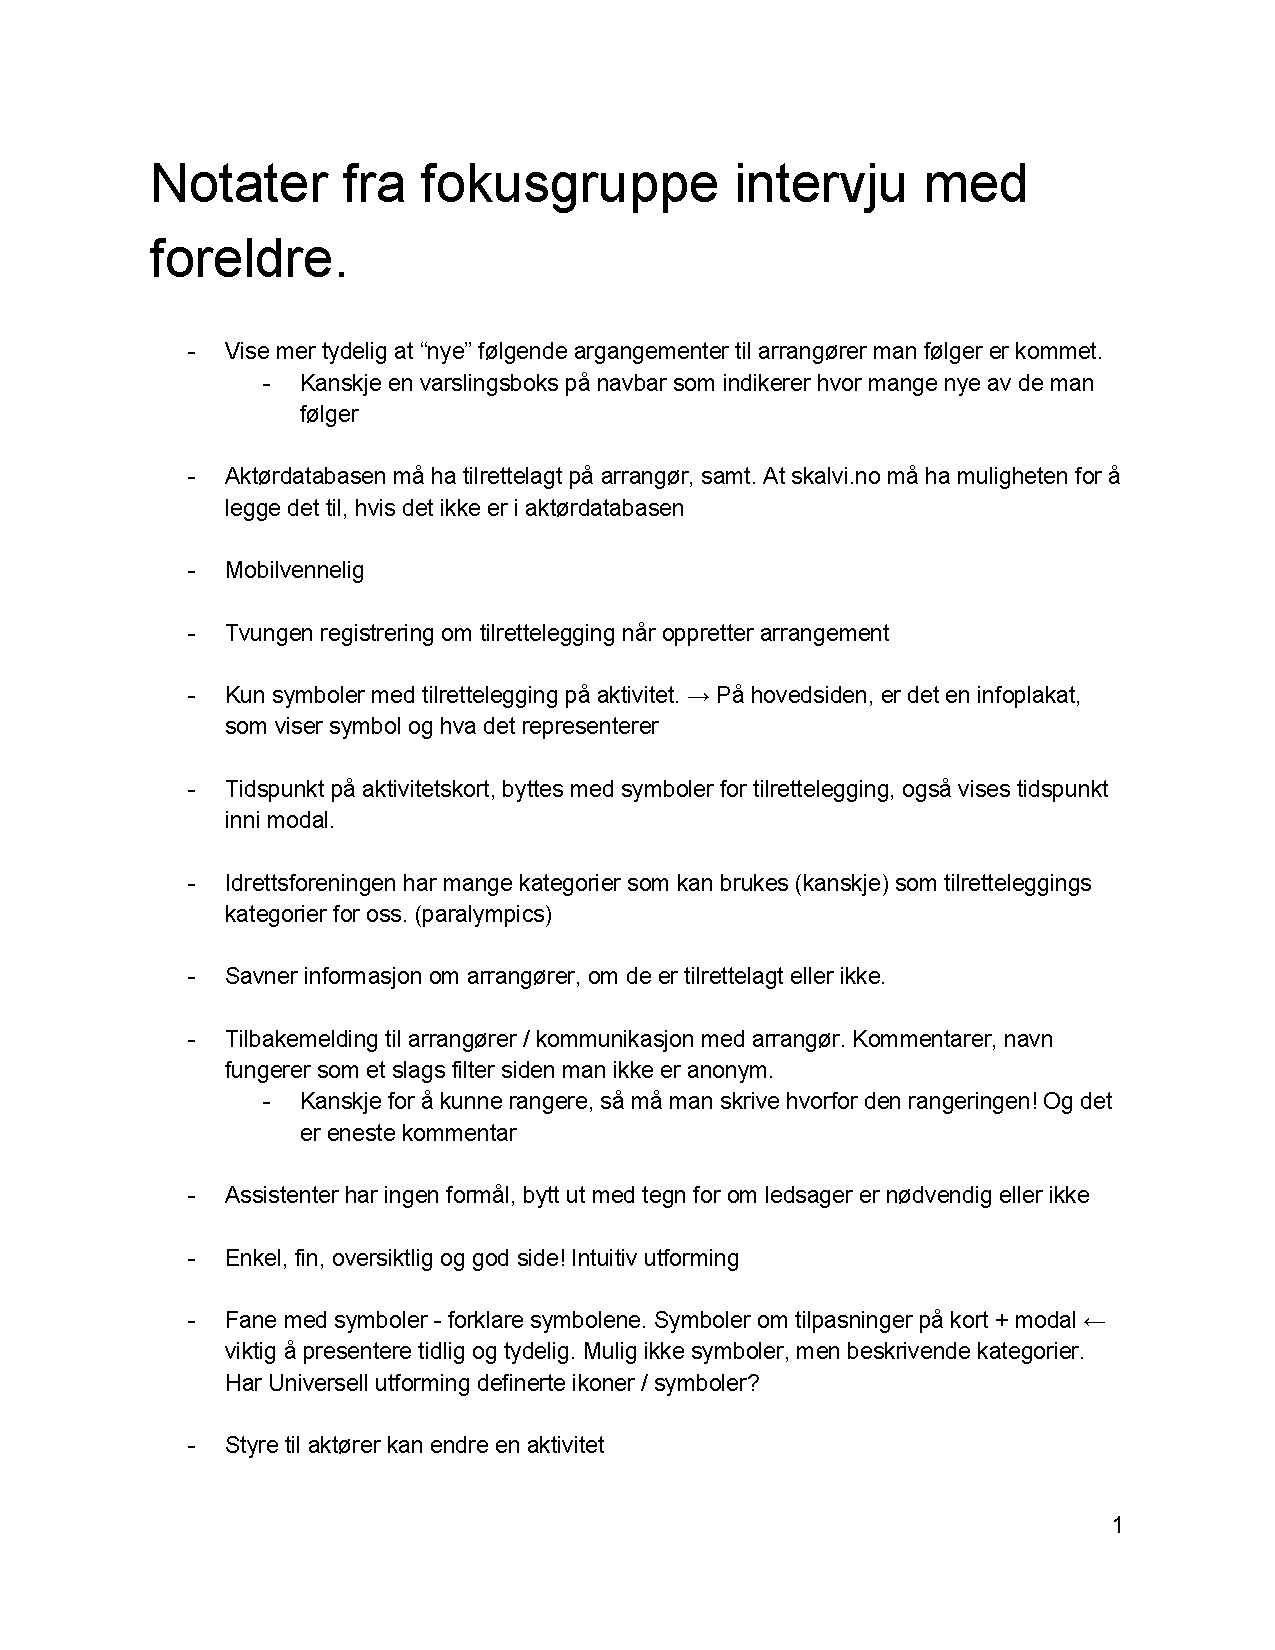
\includepdf[scale=0.9, pagecommand=\subsection{Parents}]{fig/focusgroup/FGParents_1.pdf}

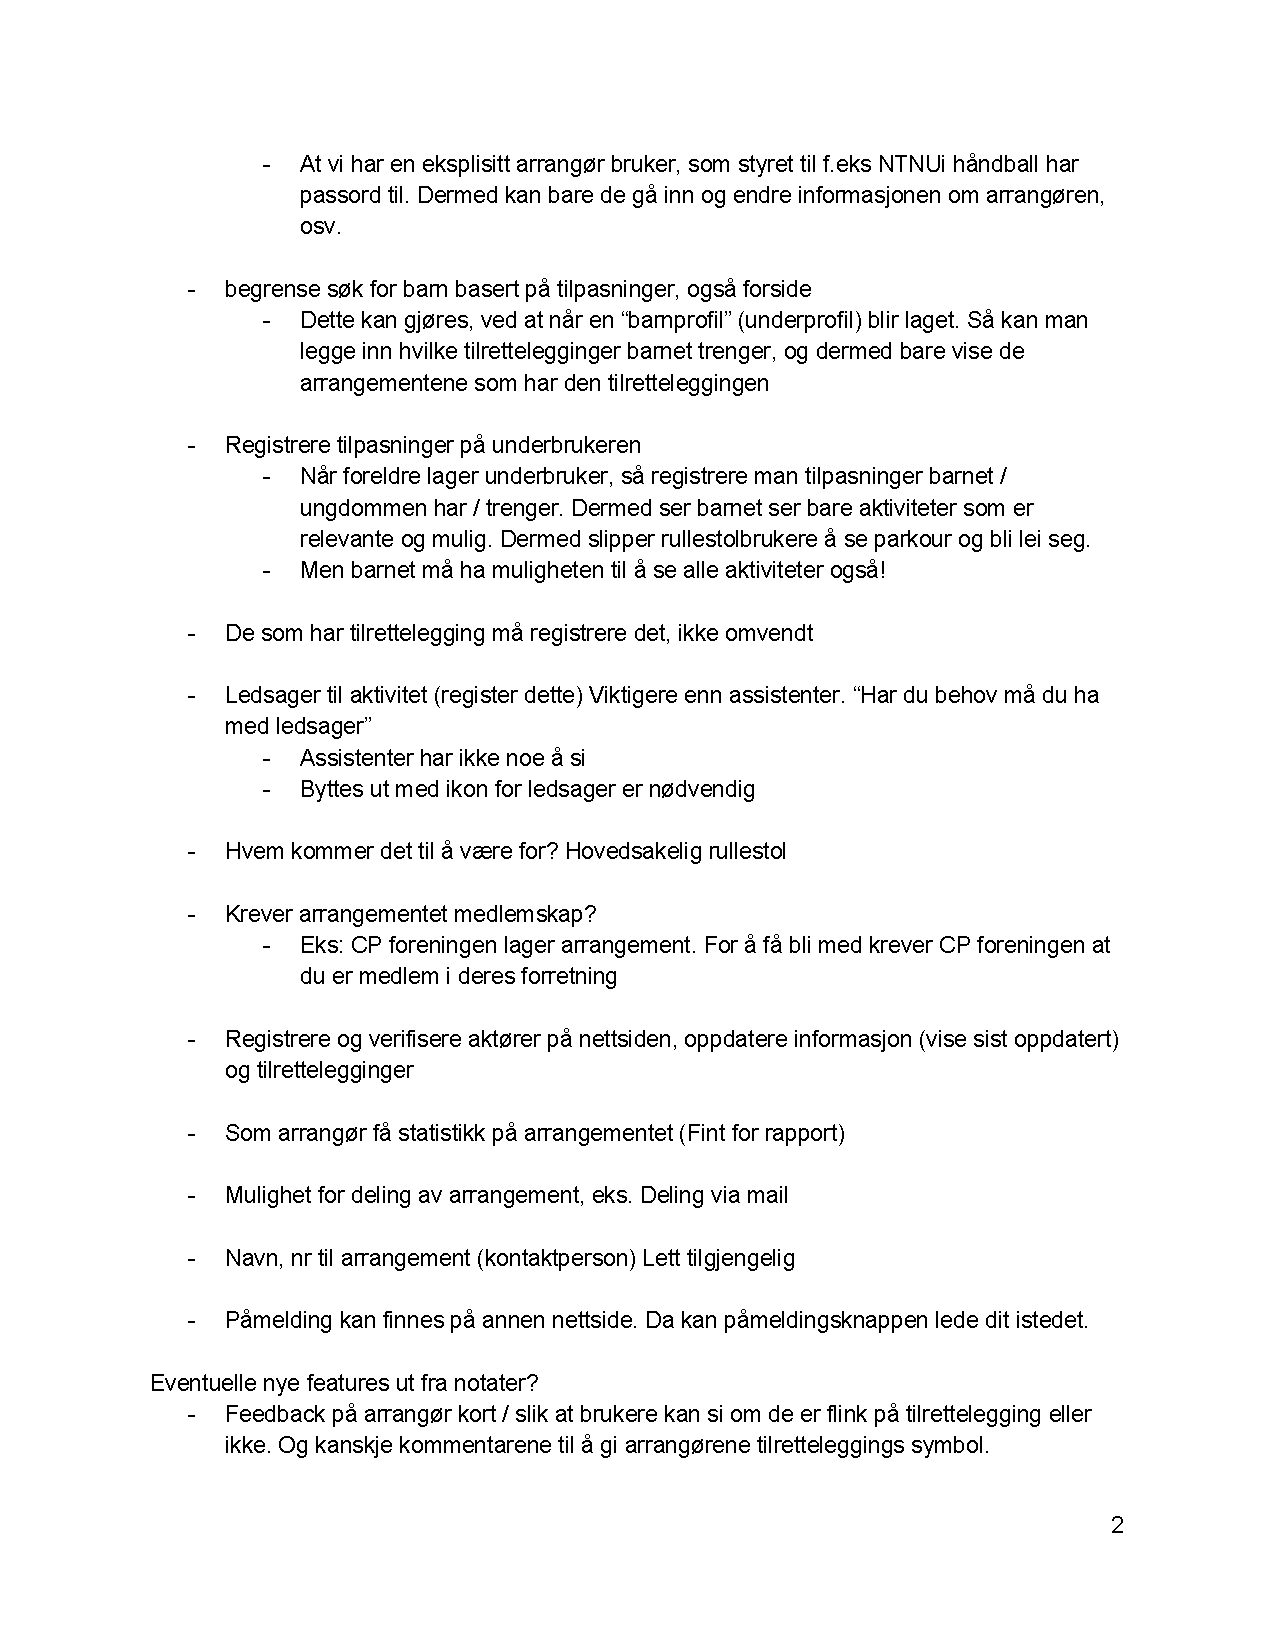
\includepdf[scale=0.9]{fig/focusgroup/FGParents_2.pdf}



\clearpage